% Aula de eletrost�tica para o curso de F\'isica II da gradua\c c\~ao
%
\documentclass[brazil,aspectratio=169]{beamer}
%
%carregando pre\^ambulo
% Standard packages

\usepackage{times}
\usepackage{polyglossia}
\usepackage{fontspec}
\usepackage[T1]{fontenc}
%\usepackage[portuguese]{babel}
\usepackage{subcaption}
\usepackage{enumitem}
\usepackage{graphicx}
\usepackage[justifying]{ragged2e}
\usepackage{multicol}
\usepackage{color}
\usepackage{mathtools}
\usepackage{hyperref}
\usepackage{cancel}
\usepackage{pifont}
\usepackage[output-decimal-marker={,}]{siunitx}
%\usepackage{animate}
\usepackage{tikz}
%\usepackage{geometry}
\usepackage{pgfplots,tikz-3dplot,circuitikz,bm,tkz-euclide,tkz-linknodes}
\usepackage{tkz-fct,tkz-base}

% Setup appearance:

\usetheme{Ilmenau}
\usefonttheme[onlylarge]{structurebold}
\setbeamerfont*{frametitle}{size=\normalsize,series=\bfseries}
\setbeamertemplate{navigation symbols}{}
\setbeamercovered{transparent}
\setlength{\columnseprule}{1pt} 
\def\columnseprulecolor{\color{blue}} 
%\setmainlanguage{portuges}
\setdefaultlanguage{portuges}

%%%%%%%%%%%%%%%%%%%%%%%%%%%%%% LyX specific LaTeX commands.
\DeclareRobustCommand{\greektext}{%
\fontencoding{LGR}\selectfont\def\encodingdefault{LGR}}
\DeclareRobustCommand{\textgreek}[1]{\leavevmode{\greektext #1}}
\DeclareFontEncoding{LGR}{}{}
\DeclareTextSymbol{\~}{LGR}{126}

% Setup new commands:

\renewcommand{\raggedright}{\leftskip=0pt \rightskip=0pt plus 0cm} 

\newcommand\Warning{%
 \makebox[1.4em][c]{%
 \makebox[0pt][c]{\raisebox{.1em}{\small\textrm{!}}}%
 \makebox[0pt][c]{\color{red}\Large$\bigtriangleup$}}}%

\newcommand\doubt{%
 \makebox[1.4em][c]{%
 \makebox[0pt][c]{\small?}%
 \makebox[0pt][c]{\raisebox{.1em}{\color{red}\Large$\bigtriangledown$}}}}%

\newcommand{\eye}[4]% size, x, y, rotation
{   \draw[rotate around={#4:(#2,#3)}] (#2,#3) -- ++(-.5*55:#1) (#2,#3) -- ++(.5*55:#1);
	\draw (#2,#3) ++(#4+55:.75*#1) arc (#4+55:#4-55:.75*#1);
	% IRIS
	\draw[fill=gray] (#2,#3) ++(#4+55/3:.75*#1) arc (#4+180-55:#4+180+55:.28*#1);
	%PUPIL, a filled arc 
	\draw[fill=black] (#2,#3) ++(#4+55/3:.75*#1) arc (#4+55/3:#4-55/3:.75*#1);
}

% Setup TikZ

\usepgfplotslibrary{fillbetween}
\usetikzlibrary{arrows,3d,calc,shadows,patterns,math,fit,shapes,optics,hobby}
\usetikzlibrary{automata,positioning,math,fit}
\usepgfplotslibrary{fillbetween}

\tikzset{>=stealth, thick, global scale/.style={scale=#1,every node/.style={scale=#1}}}
\tikzset{mid arrow/.style={postaction={decorate,decoration={markings,mark=at position .5 with {\arrow[#1]{stealth}}}}}}

\usetkzobj{all}

\pgfplotsset{compat=1.15}

% Setup paths

\graphicspath{{imagens/}}

%Autor

\author[Prof. Flaviano W. Fernandes]
{\textcolor{green!50!black}{Flaviano Williams Fernandes}}

\institute[IFPR-Irati]
{Instituto Federal do Paran� \\ Campus Irati}

\justifying


\usepackage{pst-electricfield}

%T\'itulo

\title[Eletricidade-PEL]{Potencial el\'etrico}

% The main document

\begin{document}

\begin{frame}
  \titlepage
\end{frame}

\begin{frame}{Sum\'ario}
  \tableofcontents
\end{frame}

\section{Trabalho, energia e potencial el\'etrico}

\subsection{}

\begin{frame}[fragile]{Energia potencial el\'etrica}
	\begin{columns}
		\begin{column}[c]{0.7\textwidth}
			Considere uma part\'icula carregada eletricamente no espa\c co que sofre a a\c c\~ao de uma for\c ca coulombiana devido a outro objeto carregado. Sabendo que a for\c ca \'e conservativa, temos que o trabalho W realizado por essa for\c ca para deslocar a part\'icula de um ponto i a outro ponto f \'e dado por
			\begin{align*}
				W & = -\Delta U,\\
				W & = U_i-U_f.
			\end{align*}
		\end{column}
		\begin{column}[c]{0.3\textwidth}
			\begin{figure}
				\centering
				\begin{tikzpicture}[scale=0.65, auto, transform shape, samples=50]
				
				%eixos
				\draw[line width=1.0pt,->] (0,0) -- (5,0) node[right] {x};
				\draw[line width=1.0pt,->] (0,0) -- (0,5) node[above] {y};
				
				%curva
				\pgfmathdeclarefunction{ff}{1}{\pgfmathparse{5-4/#1}}
				\pgfmathdeclarefunction{ff2}{1}{\pgfmathparse{4/(5-#1)}}
				
				%area
				%	\fill[shade] plot [domain=4:1] (\x,{ff2(\x)}) -- plot [domain=1:4] (\x,{ff(\x)});
				
				%curva
				\draw[line width=1.5pt,domain=1:2,variable=\x] plot (\x,{ff(\x)}) node [above left] {(1)};
				\draw[line width=1.5pt,domain=4:3,variable=\x] plot (\x,{ff2(\x)}) node [below right] {(2)};
				\draw[line width=1.5pt,domain=1:4,variable=\x,color=red,->] plot (\x,{ff(\x)});
				\draw[line width=1.5pt,domain=4:1,variable=\x,color=red,->] plot (\x,{ff2(\x)});
				
				%estados termodinamicos
				\node (e1) at (1,{ff(1)}) {};
				\node (e2) at (4,{ff(4)}) {};
				
				\filldraw (e1) circle (1.5pt) node[above left] {i};
				\filldraw (e2) circle (1.5pt) node[above] {f};
				
				%coordenadas
				\node[below] (vf) at (1,0) {$x_{i}$};
				\draw[dashed] (1,0) -- (e1);
				\node[below] (vi) at (4,0) {$x_{f}$};
				\draw[dashed] (4,0) -- (e2);
				
				\node[left] (pi) at (0,1) {$y_{i}$};
				\draw[dashed] (0,1) -- (e1);
				\node[left] (pf) at (0,4) {$y_{f}$};
				\draw[dashed] (0,4) -- (e2);
				
				%texto
				\node  at ($0.5*(e2)+0.5*(e1)$) {$\Delta U=0$};
				
				\end{tikzpicture}
				\caption*{\footnotesize Posi\c c\~oes inicial (i) e final (f) de uma carga no plano xy.}
			\end{figure}
		\end{column}
	\end{columns}
\end{frame}

\begin{frame}{Rela\c c\~ao entre potencial el\'etrico e trabalho}
	\begin{columns}
		\begin{column}[c]{0.6\textwidth}
			Definimos potencial el\'etrico V como o trabalho necess\'ario para deslocar cada unidade de carga do infinito at\'e o ponto P qualquer,
			\begin{align*}
			V & = \frac{W_{\infty}}{q} = \frac{U_P-U_{\infty}}{q},\\
			V & = \frac{U_P}{q},
			\end{align*}
			onde consideramos que $U_{\infty}=0$.
			\begin{block}{Potencial el\'etrico}
				Energia potencial por unidade de carga.
			\end{block}
		\end{column}
		\begin{column}[c]{0.4\textwidth}
			\begin{figure}
				\begin{tikzpicture}[scale=0.5,transform shape,font=\Large]
				
				\tkzInit[xmin=0,xmax=8,ymin=0,ymax=10]
				%\tkzGrid[color=gray!20]
				
				\tkzDefPoints{1/9/i,7/1/f,1/4/c1,5.4/6/c2}
				
				\tkzDrawPoints(i,f)
				\tkzLabelPoints[above](i)
				\tkzLabelPoints(f)
				
				\draw[dashed] (i) .. controls (c1) and (c2) .. (f);
				
				\tkzDefPoints{5/4/q}
				
				\draw[->,color=red,line width=1.0pt] (q) --++ (0,-2) node [below] {$\vec{F}$};
				\draw[->,color=red,line width=1.0pt] (q) --++ (0.6,-0.6) node [above right] {$\vec{ds}$};
				
				\draw node [draw, circle,font=\normalsize,opacity=100,fill=white] at (q) {q};
				
				\tkzDefPoints{6/8/t1,2/6/p2}
				
				\draw[->] (t1) -- (p2);
				
				\tkzText[fill=white](t1){Trajet\'oria};
				
				\end{tikzpicture}
				\caption*{\footnotesize Trajet\'oria de q do ponto i ao f.}
			\end{figure}
		\end{column}
	\end{columns}
\end{frame}

\begin{frame}{Rela\c c\~ao entre energia potencial e potencial el\'etrico}
	Quando colocamos uma part\'icula de carga q em um ponto onde j\'a existe um potencial el\'etrico V, a energia potencial da configura\c c\~ao \'e dada pela seguinte equa\c c\~ao:
	\begin{align*}
		U & = qV,\\
		\Aboxed{\text{(Energia potencial el\'etrica)} & = \text{(carga el\'etrica)}\times\text{(potencial el\'etrico)}.}
	\end{align*}
	\begin{block}{Considera\c c\~oes importantes}
		\begin{enumerate}
			\item [\ding{51}] A energia potencial el\'etrica e potencial el\'etrico est\~ao diretamente relacionados, mas s\~ao muito diferentes, e uma n\~ao pode ser usada no lugar da outra;
			\item [\ding{51}] O potencial el\'etrico n\~ao \'e um vetor, como o campo el\'etrico, e sim um escalar.
		\end{enumerate}
	\end{block}
\end{frame}

\begin{frame}{Diferen\c ca de potencial e deslocamento de cargas el\'etricas}
	\begin{columns}
		\begin{column}[c]{0.5\textwidth}
			Sabemos que $U=qV$ e $W=U_i-U_f$, podemos dizer que
			\begin{align*}
%				U_i-U_f & = W,\\
				U_i-U_f & = qV_i-qV_f,\\
				\Aboxed{\Delta V & = \frac{\Delta U}{q}=\frac{-W}{q}.}
			\end{align*}
		\end{column}
		\begin{column}[c]{0.5\textwidth}
%\begin{equation*}
%\Delta V = \frac{\Delta U}{q}.
%\end{equation*}
\begin{corollary}
	\begin{enumerate}
		\item [\ding{51}] A diferen\c ca de potencial (ddp) entre dois pontos no espa\c co \'e igual \`a diferen\c ca entre os potenciais el\'etricos dos dois pontos;
		\item [\ding{51}] A unidade de medida do potencial e da ddp no SI \'e o Volt (V), ou $N\cdot m/C$.
	\end{enumerate}
\end{corollary}
		\end{column}
	\end{columns}
	\begin{block}{El\'etron-volt}
		Muito utilizado em sistemas subat\^omicos, \'e a energia igual ao trabalho necess\'ario para deslocar uma carga elementar $e$, atrav\'es de uma ddp de um volt.
	\end{block}
\end{frame}

\begin{frame}{Superf\'icie equipotencial}
	Pontos vizinhos que possuem o mesmo potencial el\'etrico formam o que chamamos de superf\'icie equipotencial.
	\begin{columns}
		\begin{column}[c]{0.65\textwidth}
			\begin{enumerate}
				\item [\ding{51}] O trabalho realizado ao longo de uma trajet\'oria que se mant\'em em uma superf\'icie equipotencial \'e nulo (I);
				\item[\ding{51}] O trabalho realizado ao longo de uma trajet\'oria que come\c ca e termina na mesma superf\'icie equipotencial \'e nulo (II);
				\item[\ding{51}] Os trabalhos realizados ao longo de trajet\'orias que come\c cam e terminam nas mesmas superf\'icies equipotenciais s\~ao iguais (III e IV).
			\end{enumerate}
		\end{column}
		\begin{column}[c]{0.35\textwidth}
			\begin{figure}
				\begin{tikzpicture}[scale=0.42, transform shape,font=\large]
				
				\pgfmathsetmacro{\cubex}{8}
				\pgfmathsetmacro{\cubey}{4}
				\pgfmathsetmacro{\cubez}{9}
				
				\foreach \h in {0,1,2}{
					\draw[blue,fill=gray!30] (0,0+\h,\cubez) -- ++(\cubex,0,0) -- ++(0,0,-\cubez) -- ++(-\cubex,0,0) -- cycle;}
				
				\coordinate (p1) at (0,0,\cubez);
				\coordinate (p2) at (0,0+1,\cubez);
				\coordinate (p3) at (0,0+2,\cubez);
				\coordinate (p4) at (\cubex,\cubey,\cubez);
				\coordinate (p5) at (\cubex-2,\cubey,\cubez+2);
				\coordinate (p6) at (\cubex,0+2,\cubez);
				\coordinate (p7) at (\cubex,0+1,\cubez);
				\coordinate (p8) at (\cubex-2,0+1,\cubez);
				\coordinate (p9) at (\cubex-2,0+2,\cubez);
				\coordinate (p10) at (\cubex,0,\cubez);
				
				\tkzDrawPoints[size=0.3cm](p1,p2,p3,p4,p5,p6,p7,p8,p9)
				%\tkzLabelPoints(p1,p2,p3,p4,p5,p6,p7,p8,p9)
				
				\draw[<-,line width=1.0pt,color=red] (p10) arc (-90:90:0.5cm and 0.5cm) node [right,midway] {IV};
				\draw[<-,line width=1.0pt,color=red] (p1) arc (270:90:0.5cm and 0.5cm) node [left,midway] {III};
				\draw[<-,line width=1.0pt,color=red] (p7) arc (-90:90:0.5cm and 0.5cm) node [right,midway] {II};
				\draw[->,line width=1.0pt,color=red] (p8) arc (270:90:0.5cm and 0.5cm) node [left,midway] {II};
				\draw[-,line width=1.0pt,color=red] (p7) -- (p8) node [above,midway] {II};
				\draw[->,line width=1.0pt,color=red] (p4) -- (p5) node [above left,midway] {I};
				
				\end{tikzpicture}
				\caption*{\footnotesize Fam\'ilia de superf\'icies equipotenciais.}
			\end{figure}
		\end{column}
	\end{columns}
\end{frame}

\begin{frame}{Fam\'ilia de superf\'icies equipotenciais de part\'iculas puntiformes}
	\begin{figure}
		\begin{subfigure}[c]{0.45\textwidth}
			\centering
			\begin{pspicture*}(-2.5,-2.5)(2.5,2.5)
			\psscalebox{0.8}{%
				\psElectricfield[Q={[1 0 0]},linecolor=black]
				\psEquipotential[Q={[1 0 0]},
				linecolor=red,linestyle=dashed](-6.1,-6.1)(6.1,6.1)
				\psEquipotential[Q={[1 0 0]},				linecolor=white,linewidth=0\pslinewidth,Vmax=0,Vmin=0,linestyle=dashed](-6.1,-6.1)(6.1,6.1)}
			\end{pspicture*}
			\caption*{\footnotesize Carga positiva.}
		\end{subfigure}
		\begin{subfigure}[c]{0.45\textwidth}
			\centering
			\begin{pspicture*}(-2.5,-2.5)(2.5,2.5)
			\psscalebox{0.8}{%
				\psElectricfield[Q={[-1 0 0]},linecolor=black]
				\psEquipotential[Q={[-1 0 0]},
				linecolor=red,linestyle=dashed](-6.1,-6.1)(6.1,6.1)
				\psEquipotential[Q={[-1 0 0]},				linecolor=white,linewidth=0\pslinewidth,Vmax=0,Vmin=0,linestyle=dashed](-6.1,-6.1)(6.1,6.1)}
			\end{pspicture*}
			\caption*{\footnotesize Carga negativa.}
		\end{subfigure}
	\end{figure}
\end{frame}

\begin{frame}{Fam\'ilia de superf\'icie equipotenciais de um par de part\'iculas}
	\begin{figure}
		\begin{subfigure}[c]{0.45\textwidth}
			\centering
			\begin{pspicture*}(-2.5,-2.5)(2.5,2.5)
			\psscalebox{0.8}{%
				\psElectricfield[Q={[-1 -2 0][1 2 0]},linecolor=black]
				\psEquipotential[Q={[-1 -2 0][1 2 0]},
				linecolor=red,linestyle=dashed](-6.1,-6.1)(6.1,6.1)
				\psEquipotential[Q={[-1 -2 0][1 2 0]},				linecolor=white,linewidth=0\pslinewidth,Vmax=0,Vmin=0,linestyle=dashed](-6.1,-6.1)(6.1,6.1)}
			\end{pspicture*}
			\caption*{\footnotesize Dipolo el\'etrico.}
		\end{subfigure}
		\begin{subfigure}[c]{0.45\textwidth}
			\centering
			\begin{pspicture*}(-2.5,-2.5)(2.5,2.5)
				\psscalebox{0.8}{%
				\psElectricfield[Q={[1 -2 0][1 2 0]},linecolor=black]
				\psEquipotential[Q={[1 -2 0][1 2 0]},
				linecolor=red,linestyle=dashed](-6.1,-6.1)(6.1,6.1)
				\psEquipotential[Q={[1 -2 0][1 2 0]},				linecolor=white,linewidth=0\pslinewidth,Vmax=0,Vmin=0,linestyle=dashed](-6.1,-6.1)(6.1,6.1)}
			\end{pspicture*}
			\caption*{\footnotesize Cargas de sinais iguais.}
		\end{subfigure}
	\end{figure}
\end{frame}

\section{Potencial e campo el\'etrico}

\subsection{}

\begin{frame}{Potencial a partir do campo el\'etrico}
	\begin{multicols}{2}
		O trabalho $dW$ realizado por uma for\c ca $\vec{F}$ afim de efetuar um deslocamento $\vec{ds}$ em uma part\'icula \'e dado por
		\begin{equation*}
			dW = \vec{F}\cdot\vec{ds}.
		\end{equation*}
		Pela Lei de Coulomb temos $\vec{F}=q\vec{E}$. Substituindo temos
		\begin{equation*}
			dW = q\vec{E}\cdot\vec{ds}.
		\end{equation*}
		Integrando ao longo de toda a trajet\'oria temos o trabalho total realizado pela for\c ca $\vec{F}$,
		\begin{equation*}
			W = q\int_{i}^{f}\vec{E}\cdot\vec{ds}.
		\end{equation*}
		Foi mostrado anteriormente que $W=-q\Delta V$, substituindo temos
		\begin{equation*}
			\boxed{V_f-V_i = -\int_{i}^{f}\vec{E}\cdot\vec{ds}.}
		\end{equation*}
	\end{multicols}
\end{frame}

\begin{frame}{Potencial Produzido por uma Part\'icula Carregada}
	\begin{multicols}{2}
		Sabemos que uma carga puntiforme Q produz linhas de campo el\'etrico radiais, ou seja, $\vec{E}=K\frac{Q}{r^2}\widehat{r}$. Substituindo na express\~ao de $\Delta V$ obtida anteriormente encontramos
		\begin{equation*}
			V_f-V_i = -\int_{i}^{f}K\frac{Q}{r^2}dr,
		\end{equation*}
		\begin{equation*}
			V_f-V_i = \frac{Q}{4\pi\varepsilon_0}\left[\frac{1}{r}\right]_{R_i}^{R_f}.
		\end{equation*}
		Supondo que a part\'icula partiu do infinito podemos considerar $R_i=\infty$ e  $V_i=0$,
		\begin{equation*}
			\boxed{V(r) = \frac{1}{4\pi\varepsilon_0}\frac{Q}{r}.}
		\end{equation*}
	\end{multicols}
	\begin{corollary}
		O valor relativo do potencial el\'etrico depende do sinal da carga el\'etrica.
	\end{corollary}
\end{frame}

\begin{frame}{Campo el\'etrico a partir do potencial}
	\begin{multicols}{2}
		O trabalho necess\'ario para mover uma carga q em um deslocamento $d\vec{s}$ de uma superf\'icie equipotencial a outra \'e dado por $-qdV$, ou na forma $q\vec{E}\cdot d\vec{s}$, portanto
		\begin{equation*}
			-qdV=q\vec{E}\cdot d\vec{s}.
		\end{equation*}
		Usando a regra diferencial temos
		\begin{equation*}
			Ecos\theta = -\frac{dV}{ds}.
		\end{equation*}
%		Sendo $Ecos\theta$ a proje\c c\~ao de $\vec{E}$ em $d\vec{s}$ temos
%		\begin{equation*}
%			E_s=-\frac{dV}{ds}.
%		\end{equation*}
		Se considerarmos o vetor posi\c c\~ao como $\vec{s}=x\widehat{i}+y\widehat{j}+z\widehat{k}$ e $s=\sqrt{x^2+y^2+z^2}$ podemos determinar as componentes de $\vec{E}$ na dire\c c\~ao x usando a regra da cadeia,
		\begin{align*}
			\frac{\partial V}{\partial x} & =\frac{dV}{ds}\frac{\partial s}{\partial x}=\left(-Ecos\theta\right)\left(\frac{x}{s}\right),\\
			\frac{\partial V}{\partial x} & =-\vec{E}\cdot\widehat{i}=-E_x.
		\end{align*}
		Usando o mesmo racioc\'inio nas dire\c c\~oes y e z temos
	\begin{equation*}
		\boxed{E_x=-\frac{\partial V}{\partial x},\quad E_y=-\frac{\partial V}{\partial y},\quad E_z=-\frac{\partial V}{\partial z}.}
	\end{equation*}
	\end{multicols}
\end{frame}

\section{Potencial de uma distribui\c c\~ao de cargas}

\subsection{}

\begin{frame}{Potencial de uma distribui\c c\~ao discreta de cargas}
	\begin{columns}
		\begin{column}[c]{0.5\textwidth}
			\begin{figure}
				\centering
				\begin{tiny}
					\tdplotsetmaincoords{70}{110}
					\begin{tikzpicture}[scale=3, tdplot_main_coords,
						axis/.style={->,blue,thick},
						vectora/.style={<->,thick},
						vectorb/.style={<->,red,thick}]
		
						%standard tikz coordinate definition using x, y, z coords
						\coordinate (O) at (0,0,0);
		
						%draw axes
						\draw[axis] (0,0,0) -- (1,0,0) node[anchor=north east]{$x$};
						\draw[axis] (0,0,0) -- (0,1,0) node[anchor=north west]{$y$};
						\draw[axis] (0,0,0) -- (0,0,1) node[anchor=south]{$z$};
		
						%configurando estilo das cargas
						\tikzstyle{s1}=[tdplot_screen_coords, circle, radius=0.001, ball color=gray!50];
						\tikzstyle{s2}=[tdplot_screen_coords, right];
		
						%draw charges
						\tdplottransformmainscreen{0.3}{0.5}{1.}
						\node [s1] (n1) at (\tdplotresx,\tdplotresy) {$q_{1}$};
		
						\tdplottransformmainscreen{0.3}{-0.5}{0.1}
						\node [s1] (n2) at (\tdplotresx,\tdplotresy) {$q_{2}$};
		
						\tdplottransformmainscreen{0.6}{-0.4}{1.}
						\node [s1] (n3) at (\tdplotresx,\tdplotresy) {$q_{3}$};
		
						\tdplottransformmainscreen{0.9}{0.8}{0.1}
						\node [s1] (n4) at (\tdplotresx,\tdplotresy) {$q_{4}$};
		
						\tdplottransformmainscreen{1.3}{0.4}{0.1}
						\node [s1] (n5) at (\tdplotresx,\tdplotresy) {$q_{5}$};
		
						\tdplottransformmainscreen{0.9}{0.9}{0.7}
						\node [s2] (ni) at (\tdplotresx,\tdplotresy) {$P$};
		
						%\tdplottransformmainscreen{1.0}{1.0}{1.5}
						%\node [s2] (t1) at (\tdplotresx,\tdplotresy) {\normalsize carga de prova};
		
						%draw a vector from origin to charge
						%\draw[vectora] (O) -- (n1) node[above,midway] {$r_{1}$};
		
						%draw a vector from origin to charge
						%\draw[vectora] (O) -- (n2) node[above,midway] {$r_{2}$};
		
						%draw a vector from origin to charge
						%\draw[vectora] (O) -- (n3) node[above,midway] {$r_{3}$};
		
						%draw a vector from origin to charge
						%\draw[vectora] (O) -- (n4) node[above,midway] {$r_{4}$};
		
						%draw a vector from origin to charge
						%\draw[vectora] (O) -- (n5) node[right,midway] {$r_{5}$};
		
						%draw a vector from origin to charge
						%\draw[vectora] (O) -- (ni) node[above,midway] {$r_{i}$};
		
						%draw a vector from origin to charge
						\draw[vectorb] (n1) -- (ni) node[right,midway] {$r_{1P}$};
		
						%draw a vector from origin to charge
						\draw[vectorb] (n2) -- (ni) node[above,midway] {$r_{2P}$};
		
						%draw a vector from origin to charge
						\draw[vectorb] (n3) -- (ni) node[above,midway] {$r_{3P}$};
		
						%draw a vector from origin to charge
						\draw[vectorb] (n4) -- (ni) node[right,midway] {$r_{4P}$};
		
						%draw a vector from origin to charge
						\draw[vectorb] (n5) -- (ni) node[above,midway] {$r_{5P}$};
		
						%draw a vector from origin to charge
%						\draw[red,->,line width=1.5pt] (t1) -- (ni);
		
					\end{tikzpicture}
				\end{tiny}
				%\tdplotsetmaincoords{70}{110}
\begin{tikzpicture}[scale=3, tdplot_main_coords,
					axis/.style={->,blue,thick},
					vectora/.style={-stealth,thick},
					vectorb/.style={-stealth,red,thick}]

	%standard tikz coordinate definition using x, y, z coords
	\coordinate (O) at (0,0,0);
	
	%draw axes
	\draw[axis] (0,0,0) -- (1,0,0) node[anchor=north east]{$x$};
	\draw[axis] (0,0,0) -- (0,1,0) node[anchor=north west]{$y$};
	\draw[axis] (0,0,0) -- (0,0,1) node[anchor=south]{$z$};
	
	%configurando estilo das cargas
	\tikzstyle{s1}=[tdplot_screen_coords, circle, radius=0.005, ball color=gray];
	\tikzstyle{s2}=[tdplot_screen_coords, right];

	%draw charges
	\tdplottransformmainscreen{0.3}{0.5}{1.}
	\node [s1] (n1) at (\tdplotresx,\tdplotresy) {$q_{1}$};

	\tdplottransformmainscreen{0.3}{-0.5}{0.1}
	\node [s1] (n2) at (\tdplotresx,\tdplotresy) {$q_{2}$};

	\tdplottransformmainscreen{0.6}{-0.4}{1.}
	\node [s1] (n3) at (\tdplotresx,\tdplotresy) {$q_{3}$};

	\tdplottransformmainscreen{0.9}{0.8}{0.1}
	\node [s1] (n4) at (\tdplotresx,\tdplotresy) {$q_{4}$};

	\tdplottransformmainscreen{1.3}{0.4}{0.1}
	\node [s1] (n5) at (\tdplotresx,\tdplotresy) {$q_{5}$};

	\tdplottransformmainscreen{0.9}{0.9}{0.7}
	\node [s1] (ni) at (\tdplotresx,\tdplotresy) {$q_{i}$};

	\tdplottransformmainscreen{1.0}{1.0}{1.5}
	\node [s2] (t1) at (\tdplotresx,\tdplotresy) {\normalsize Carga de prova};

	%draw a vector from origin to charge
	\draw[vectora] (O) -- (n1) node[above,midway] {$\vec{r}_{1}$};
	
	%draw a vector from origin to charge
	\draw[vectora] (O) -- (n2) node[above,midway] {$\vec{r}_{2}$};
	
	%draw a vector from origin to charge
	\draw[vectora] (O) -- (n3) node[above,midway] {$\vec{r}_{3}$};
	
	%draw a vector from origin to charge
	\draw[vectora] (O) -- (n4) node[above,midway] {$\vec{r}_{4}$};
	
	%draw a vector from origin to charge
	\draw[vectora] (O) -- (n5) node[right,midway] {$\vec{r}_{5}$};
	
	%draw a vector from origin to charge
	\draw[vectora] (O) -- (ni) node[above,midway] {$\vec{r}_{i}$};
	
	%draw a vector from origin to charge
	\draw[vectorb] (n1) -- (ni) node[right,midway] {$\vec{r}_{1i}$};
	
	%draw a vector from origin to charge
	\draw[vectorb] (n2) -- (ni) node[above,midway] {$\vec{r}_{2i}$};
	
	%draw a vector from origin to charge
	\draw[vectorb] (n3) -- (ni) node[above,midway] {$\vec{r}_{3i}$};
	
	%draw a vector from origin to charge
	\draw[vectorb] (n4) -- (ni) node[right,midway] {$\vec{r}_{4i}$};
	
	%draw a vector from origin to charge
	\draw[vectorb] (n5) -- (ni) node[above,midway] {$\vec{r}_{5i}$};
	
	%draw a vector from origin to charge
	\draw[red,->,line width=1.5pt] (t1) -- (ni);
	
\end{tikzpicture}

				\caption*{\footnotesize Dist\^ancia relativa entre cargas $q$ e o ponto P.}
			\end{figure}
		\end{column}
		\begin{column}[c]{0.5\textwidth}
			Podemos calcular o potencial no ponto P produzido por uma distribui\c c\~ao de cargas usando o princ\'ipio da superposi\c c\~ao,
			\begin{equation*}
				V=V_1+V_2+\cdots+V_N.
			\end{equation*}
			\begin{block}{Potencial el\'etrico de uma distribui\c c\~ao puntiforme de cargas el\'etricas}
				\[V = \frac{1}{4\pi\varepsilon_0}\sum_{i=1}^{N}\frac{Q_{i}}{r_{i}}\]
			\end{block}
		\end{column}
	\end{columns}
\end{frame}

\begin{frame}{Potencial Produzido por um dipolo el\'etrico}
	\begin{columns}
		\begin{column}[t]{0.6\textwidth}
			Na figura ao lado, o potencial el\'etrico em um ponto P \'e dado pela soma dos potenciais produzidos pelas duas cargas,
			\begin{align*}
				V & = V_++V_-,\\
				V & = \frac{1}{4\pi\varepsilon_0}\left(\frac{+q}{r_+}+\frac{-q}{r_-}\right),\\
				V & = \frac{q}{4\pi\varepsilon_0}\frac{(r_--r_+)}{r_-r_+}.
			\end{align*}
		\end{column}
		\begin{column}[t]{0.4\textwidth}
			\begin{figure}
%				\vspace*{-1cm}
				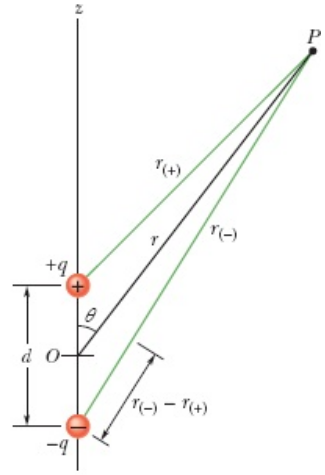
\includegraphics[scale=0.25]{figuras/figura-1.png}
				\caption*{\footnotesize Potencial no ponto O devido a um dipolo el\'etrico.}
			\end{figure}
		\end{column}
	\end{columns}
\end{frame}

\begin{frame}{Potencial Produzido por um dipolo el\'etrico (continua\c c\~ao)}
	\begin{columns}
		\begin{column}[t]{0.6\textwidth}
			Se considerarmos pontos relativamente distantes do dipolo, onde $r>>d$, podemos dizer que $r_-\approx r_+\approx r$ e
			\begin{align*}
				r_--r_+ = dcos\theta,\quad r_-r_+ = r^2.
			\end{align*}
			Substituindo na express\~ao do potencial e definindo o momento de dipolo $p=qd$, temos
			\begin{align*}
				V & = \frac{q}{4\pi\varepsilon_0}\frac{dcos\theta}{r^2},\\
				\Aboxed{V & = \frac{1}{4\pi\varepsilon_0}\frac{pcos\theta}{r^2}.}
			\end{align*}
		\end{column}
		\begin{column}[t]{0.4\textwidth}
			\begin{figure}
%				\vspace*{-1cm}
				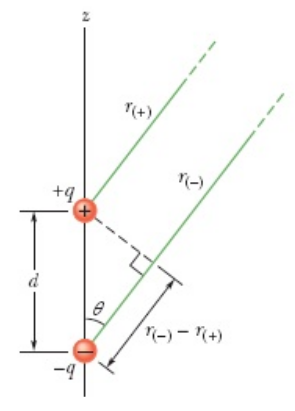
\includegraphics[scale=0.29]{figuras/figura-2.png}
				\caption*{\footnotesize $r_+$ e $r_-$ s\~ao praticamente paralelos se $r>>d$.}
			\end{figure}
		\end{column}
	\end{columns}
\end{frame}

\begin{frame}{Potencial de uma distribui\c c\~ao cont\'inua de cargas}
	\begin{multicols}{2}
		Tratando o elemento de carga dq como uma carga pontual, podemos usar a seguinte express\~ao para expressar o potencial dV no ponto P produzido por dq,
		\begin{equation*}
			dV=\frac{1}{4\pi\varepsilon_0}\frac{dq}{r},
		\end{equation*}
		onde r \'e a dist\^ancia entre P e a carga dq.\linebreak
		Para calcular o potencial total V no ponto P, integramos cada contribui\c c\~ao de dq,
		\begin{equation*}
			\boxed{V=\frac{1}{4\pi\varepsilon_0}\int \frac{dq}{r}.}
		\end{equation*}
	\end{multicols}
	\begin{corollary}
		\begin{enumerate}
			\item[\ding{51}] A integral deve ser calculada para toda a distribui\c c\~ao de carga.
			\item[\ding{51}] O potencial \'e um escalar, portanto n\~ao existem componentes vetoriais a serem considerados.
		\end{enumerate}
	\end{corollary}
\end{frame}

\begin{frame}{Potencial el\'etrico de um fio retil\'ineo finito}
	\begin{columns}
		\begin{column}[c]{0.65\textwidth}
			Considere um fio retil\'ineo contendo uma distribui\c c\~ao uniforme de carga $\lambda$. Cada peda\c co infinitesimal $dz$ do fio ter\'a uma quantidade de carga $dq$, onde o potencial no ponto P \'e dado por
			\begin{equation*}
				dq = \lambda dz.
			\end{equation*}
			Cada elemento de carga $dq$ ir\'a produzir um potencial dV id\^entico a de uma part\'icula puntiforme
			\begin{equation*}
				dV = \frac{1}{4\pi\varepsilon_0}\frac{dq}{r}.
			\end{equation*}	
		\end{column}
		\begin{column}[c]{0.35\textwidth}
			\begin{figure}
				\begin{tikzpicture}[scale=0.7,transform shape,font=\Large]
					\draw[line width=4pt,color=gray!50] (0,-3) -- (0,3) node [midway] (l1) {};
					\coordinate (p1) at (2,0);
					\coordinate (p2) at (0.0,-2);
					\foreach \x in {-3,-2.5,...,3}
					\node[left] at(0,\x) {$+$};
					\filldraw (p1) circle (1.5pt) node[right] (n1) at (2,0) {P};
					\draw[dotted] (l1) -- (p1) node [midway,above] {$d$};
					\draw[dotted] (p2) -- (p1) node [midway,below right] {$r$};
					\draw ($(p2)+(0,-0.25)$) to [short dim arrow'={label'=$dz$}] ($(p2)+(0,0.25)$);
				\end{tikzpicture}
				\caption*{\footnotesize Fio retilineo com distribui\c c\~ao uniforme de carga $\lambda$.}
			\end{figure}
		\end{column}
	\end{columns}
\end{frame}

\begin{frame}{Potencial el\'etrico de um fio retil\'ineo finito (continua\c c\~ao)}
	\begin{multicols}{2}
%	\begin{columns}
%		\begin{column}[t]{0.5\textwidth}
			Substituindo $r$ na equa\c c\~ao temos
			\begin{equation*}
				dV = \frac{1}{4\pi\varepsilon_0}\frac{\lambda dz}{\left(z^2+d^2\right)^{1/2}}.
			\end{equation*}	
			Para obter o potencial no ponto P integramos a contribui\c c\~ao de cada peda\c co $dz$ do fio,
			\begin{equation*}
				V = \frac{1}{4\pi\varepsilon_0}\int_{0}^{L} \frac{\lambda dz}{\left(z^2+d^2\right)^{1/2}}.
			\end{equation*}
			Para resolver a integral usamos a t\'ecnica do teorema de Cauchy, o que resulta em
%		\end{column}
%		\begin{column}[t]{0.5\textwidth}
			\begin{equation*}
				V = \frac{\lambda}{4\pi\varepsilon_0}\left[ln\left(x+(x^2+d^2)^{1/2}\right)\right]_{0}^{L}.
			\end{equation*}
			Usando a identidade $lnA-lnB=ln\left(A/B\right)$ chegamos ao resultado final,
			\begin{equation*}
				\boxed{V = \frac{\lambda}{4\pi\varepsilon_0}ln\left[\frac{L+(L^2+d^2)^{1/2}}{d}\right].}
			\end{equation*}
%		\end{column}
%	\end{columns}
	\end{multicols}
\end{frame}

\begin{frame}{Potencial el\'etrico de um disco carregado}
	\begin{columns}
		\begin{column}[c]{0.65\textwidth}
			Considere um disco carregado eletricamente com uma densidade superficial de carga $\sigma$. Podemos considerar que o disco \'e formado por v\'arios an\'eis de espessura $dR1$ e raio $R$ contendo cargas $dq$, onde
			\begin{align*}
				dq & = \sigma dA,\\
				dq & = \sigma 2\pi R'dR'.
			\end{align*}
			sendo $dA$ a \'area do anel. A carga total do disco \'e obtida integrando $dq$ de cada anel, ou seja,
			\begin{equation*}
				q = \int dq = \int_{0}^{R}\sigma dA = \sigma \pi R^2.
			\end{equation*}			
		\end{column}
		\begin{column}[c]{0.35\textwidth}
			\vspace*{-1cm}
			\begin{figure}
				\begin{tikzpicture}[scale=0.5,transform shape,font=\large]
					
					\tkzInit[xmin=-5,xmax=5,ymin=-1,ymax=8.5]
					%\tkzGrid[color=gray!20]
					\tkzClip
					
					\tkzDefPoints{0/0/O, 0/0.25/O', -3/0/A, 3/0/C,0/7/G,-1.5/-0.25/o',-1.75/-0.25/o1}
					\tkzDefPointsBy[translation = from O to O'](A,C){F,H}
					
					\draw[dashed,fill=blue!20,opacity=0.25] (C) arc (0:180:3cm and 1cm);
					\draw[fill=blue!20,opacity=0.25,draw opacity=100] (C) arc (0:-180:3cm and 1cm);
					\draw[fill=blue!20,opacity=0.25,draw opacity=100] (O') ellipse (3cm and 1cm);
					\draw (O') ellipse (1.5cm and 0.4cm);
					\draw (O') ellipse (1.75cm and 0.6cm);
					
					\draw[->,line width=1.0pt] (O') -- (-1,0) node [above,midway] {R'};
					\draw[->,line width=1.0pt] (O') -- (H) node [above,pos=0.75] {R};
					\draw[->,line width=1.0pt] (O') -- (G) node [right,pos=0.5] {z};
					\draw[<->,line width=1.0pt] (-1,0) -- (G) node [left,midway] {r};
					\draw (o1) to [short dim arrow={label=$dR'$}] (o');
					
					\tkzDrawPoint[color=red,size=0.4cm,fill=red](G)
					\tkzLabelPoint[right=0.1](G){P}
					
				\end{tikzpicture}
				\caption*{\footnotesize Disco circular com distribui\c c\~ao uniforme de carga.}
			\end{figure}
		\end{column}
	\end{columns}
\end{frame}

\begin{frame}{Potencial el\'etrico de um disco circular (continua\c c\~ao)}
	\begin{columns}
		\begin{column}[t]{0.5\textwidth}
			Cada anel de largura dR' ir\'a produzir um potencial dV no ponto P, onde
			\begin{align*}
				dV & = \frac{1}{4\pi\varepsilon_0}\frac{dq}{r},\\
				dV & = \frac{1}{4\pi\varepsilon_0}\frac{\sigma 2\pi R'}{\left(z^2+R'^2\right)^{1/2}}dR'.
			\end{align*}
			Integrando temos
			\begin{equation*}
				V = \frac{1}{4\pi\varepsilon_0}\int \frac{\sigma 2\pi R'}{\left(z^2+R'^2\right)^{1/2}}dR'
			\end{equation*}
		\end{column}
		\begin{column}[t]{0.5\textwidth}
			Para resolver a integral fazemos a substitui\c c\~ao $X=z^2+R'^2$ e $dX=2R'dR'$,
			\begin{align*}
				V & = \frac{1}{4\pi\varepsilon_0}\pi\sigma\int X^{-1/2}dX,\\
				V & = \frac{1}{4\pi\varepsilon_0}\overbracket{\pi\sigma}^{\alert{q/R^2}}\left[\frac{\left(z^2+R'^2\right)^{1/2}}{1/2}\right]^{R}_{0}.
			\end{align*}
			Chegamos assim na solu\c c\~ao final,
			\begin{equation*}
				\boxed{V(z) = \frac{q}{2\pi\varepsilon_0R^2}\left(\sqrt{z^2+R^2}-z\right).}
			\end{equation*}
		\end{column}
	\end{columns}
\end{frame}

\begin{frame}{Potencial el\'etrico de um condutor carregado}
	\begin{columns}
		\begin{column}[t]{0.6\textwidth}
			\begin{enumerate}
				\item [\ding{51}] Uma carga em excesso colocada em um condutor se distribui na superf\'icie do condutor de tal forma que o potencial \'e o mesmo em todos os pontos (tanto na superf\'icie quanto no interior), mesmo que o condutor tenha uma cavidade interna;
				\item[\ding{51}] As linhas de campo el\'etrico cruzam perpendicularmente as superf\'icies superficiais.
			\end{enumerate}
		\end{column}
		\begin{column}[t]{0.4\textwidth}
			\begin{figure}
				\centering
				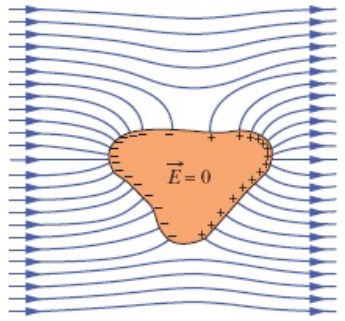
\includegraphics[scale=0.3]{figuras/figura-3.png}
				\caption*{\footnotesize Condutor descarregado inserido em um campo el\'etrico externo.}
			\end{figure}
		\end{column}
	\end{columns}
\end{frame}

\begin{frame}{Potencial el\'etrico em uma esfera condutora}
	\begin{columns}
		\begin{column}[c]{0.6\textwidth}
			Como foi visto anteriormente, o campo el\'etrico de uma esfera condutora \'e dado por
			\begin{equation*}
				\boxed{E(r) = 
				\begin{cases}
					0,\quad & (r<R),\\
					\frac{1}{4\pi\varepsilon_0}\frac{q}{r^2},\quad & (r\ge R).
				\end{cases}}
			\end{equation*}
			No caso da esfera condutora temos que o potencial \'e o mesmo no interior e na superf\'icie,
			\begin{equation*}
				\boxed{V(r) = 
				\begin{cases}
					\frac{1}{4\pi\varepsilon_0}\frac{q}{R},\quad & (r \le R),\\
					\frac{1}{4\pi\varepsilon_0}\frac{q}{r},\quad & (r > R).
				\end{cases}}
			\end{equation*}
		\end{column}
		\begin{column}[c]{0.4\textwidth}
			\begin{figure}
				\centering
				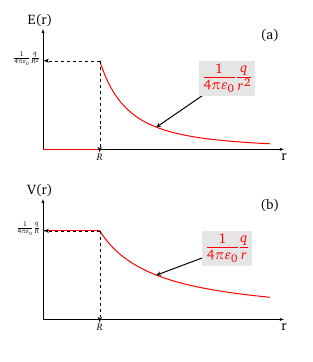
\includegraphics[scale=0.5]{figuras/potencial-esfera.png}
				\caption*{\footnotesize Campo el\'etrico (a) e potencial (b) de uma esfera condutora eletricamente carregada.}
			\end{figure}
		\end{column}
	\end{columns}
\end{frame}

\section{Ap\^endice}

\subsection{}

\begin{frame}{Transformar um n\'umero em nota\c c\~ao cient\'ifica}
	\begin{corollary}
		\begin{enumerate}[leftmargin=1.75cm]
			\item[Passo 1:] Escrever o n\'umero incluindo a v\'irgula.
			\item[Passo 2:] Andar com a v\'irgula at\'e que reste somente um n\'umero diferente de zero no lado esquerdo.
			\item[Passo 3:] Colocar no expoente da pot\^encia de 10 o n\'umero de casas decimais que tivemos que "andar" com a v\'irgula. Se ao andar com a v\'irgula o valor do n\'umero diminuiu, o expoente ficar\'a positivo, se aumentou o expoente ficar\'a negativo.
		\end{enumerate}
	\end{corollary}
	\begin{exampleblock}{Exemplo}
		\begin{equation*}
			6\; 590\; 000\; 000\; 000\; 000,0 = \SI{6,59e15}{}		
		\end{equation*}
	\end{exampleblock}
\end{frame}

\begin{frame}{Convers\~ao de unidades em uma dimens\~ao}
	\begin{figure}
		\begin{tikzpicture}[scale=0.65,transform shape,font=\Large]
		
		\tkzInit[xmin=-2,xmax=17,ymin=-6,ymax=3]
		%\tkzGrid[color=gray!20]
		\tkzClip
		
		\tikzset{compass style/.append style={->}}
		
		\foreach \x in {1,2,3}{
			\tkzDefPoint(\x*3-3,0){\x}
			\tkzDrawArc[R,line width=1.0pt](\x,1.5 cm)(20,160)
			\node at (\x*3-3,2) {$\times 10^{3}$};
			\tkzDrawArc[R,line width=1.0pt](\x,1.5 cm)(200,340)
			\node at (\x*3-3,-2) {$\times 10^{-3}$};}
		
		\foreach \x in {4,5,6}{
			\tkzDefPoint(\x*3-3,0){\x}
			\tkzDrawArc[R,line width=1.0pt](\x,1.5 cm)(20,160)
			\node at (\x*3-3,2) {$\times 10^{1}$};
			\tkzDrawArc[R,line width=1.0pt](\x,1.5 cm)(200,340)
			\node at (\x*3-3,-2) {$\times 10^{-1}$};}
		
		\tkzDefPoints{-1.5/0/p1,1.5/0/p2,4.5/0/p3,7.5/0/p4,10.5/0/p5,13.5/0/p6,16.5/0/p7}
		
		\tkzText(p1){$\si{\pico}\_^{}$}
		\tkzText(p2){$\si{\nano}\_^{}$}
		\tkzText(p3){$\si{\micro}\_^{}$}
		\tkzText(p4){$\si{m}\_^{}$}
		\tkzText(p5){$\si{\centi}\_^{}$}
		\tkzText(p6){$\si{\deci}\_^{}$}
		\tkzText(p7){$\_^{}$}
		
		%exemplos
		
		\tkzText(3,-3.5){$1\;\text{mm}=1\times 10^{(-1)\times\alert{2}}\;\text{dm}\rightarrow 1\times 10^{-2}\;\text{dm}$}
		\tkzText(3.25,-4.5){$2,5\;\text{g}=2,5\times 10^{(1)\times\alert{3}}\;\text{mg}\rightarrow2,5\times 10^{3}\;\text{mg}$}
		\tkzText(3.7,-5.5){$10\;\mu\text{C}=10\times 10^{\left[(-3)\times\alert{1}+(-1)\times\alert{3}\right]}\;\text{C}\rightarrow 10\times 10^{-6}\;\text{C}$}
		
		\end{tikzpicture}
	\end{figure}
\end{frame}

\begin{frame}{Convers\~ao de unidades em duas dimens\~oes}
	\begin{figure}
		\begin{tikzpicture}[scale=0.65,transform shape,font=\Large]
	
		\tkzInit[xmin=-2,xmax=17,ymin=-6,ymax=3]
		%\tkzGrid[color=gray!20]
		\tkzClip
	
		\tikzset{compass style/.append style={->}}
	
		\foreach \x in {1,2,3}{
			\tkzDefPoint(\x*3-3,0){\x}
			\tkzDrawArc[R,line width=1.0pt](\x,1.5 cm)(20,160)
			\node at (\x*3-3,2) {$\times 10^{6}$};
			\tkzDrawArc[R,line width=1.0pt](\x,1.5 cm)(200,340)
			\node at (\x*3-3,-2) {$\times 10^{-6}$};}
		
		\foreach \x in {4,5,6}{
			\tkzDefPoint(\x*3-3,0){\x}
			\tkzDrawArc[R,line width=1.0pt](\x,1.5 cm)(20,160)
			\node at (\x*3-3,2) {$\times 10^{2}$};
			\tkzDrawArc[R,line width=1.0pt](\x,1.5 cm)(200,340)
			\node at (\x*3-3,-2) {$\times 10^{-2}$};}
		
		\tkzDefPoints{-1.5/0/p1,1.5/0/p2,4.5/0/p3,7.5/0/p4,10.5/0/p5,13.5/0/p6,16.5/0/p7}
	
		\tkzText(p1){$\si{\pico}\_^{2}$}
		\tkzText(p2){$\si{\nano}\_^{2}$}
		\tkzText(p3){$\si{\micro}\_^{2}$}
		\tkzText(p4){$\si{m}\_^{2}$}
		\tkzText(p5){$\si{\centi}\_^{2}$}
		\tkzText(p6){$\si{\deci}\_^{2}$}
		\tkzText(p7){$\_^{2}$}
		
		%exemplos
	
		\tkzText(3.3,-3.5){$1\;\text{mm}^2=1\times 10^{(-2)\times\alert{2}}\;\text{dm}^2\rightarrow 1\times 10^{-4}\;\text{dm}^2$}
		\tkzText(3.6,-4.5){$2,5\;\text{m}^2=2,5\times 10^{(2)\times\alert{3}}\;\text{mm}^2\rightarrow2,5\times 10^{6}\;\text{mm}^2$}
		\tkzText(4.1,-5.5){$10\;\mu\text{m}^2=10\times 10^{\left[(-6)\times\alert{1}+(-2)\times\alert{3}\right]}\;\text{m}^2\rightarrow 10\times 10^{-12}\;\text{m}^2$}
	
		\end{tikzpicture}
	\end{figure}
\end{frame}

\begin{frame}{Convers\~ao de unidades em tr\^es dimens\~oes}
	\begin{figure}
		\begin{tikzpicture}[scale=0.65,transform shape,font=\Large]
	
		\tkzInit[xmin=-2,xmax=17,ymin=-6,ymax=3]
		%\tkzGrid[color=gray!20]
		\tkzClip
	
		\tikzset{compass style/.append style={->}}
	
		\foreach \x in {1,2,3}{
			\tkzDefPoint(\x*3-3,0){\x}
			\tkzDrawArc[R,line width=1.0pt](\x,1.5 cm)(20,160)
			\node at (\x*3-3,2) {$\times 10^{9}$};
			\tkzDrawArc[R,line width=1.0pt](\x,1.5 cm)(200,340)
			\node at (\x*3-3,-2) {$\times 10^{-9}$};}
		
		\foreach \x in {4,5,6}{
			\tkzDefPoint(\x*3-3,0){\x}
			\tkzDrawArc[R,line width=1.0pt](\x,1.5 cm)(20,160)
			\node at (\x*3-3,2) {$\times 10^{3}$};
			\tkzDrawArc[R,line width=1.0pt](\x,1.5 cm)(200,340)
			\node at (\x*3-3,-2) {$\times 10^{-3}$};}
		
		\tkzDefPoints{-1.5/0/p1,1.5/0/p2,4.5/0/p3,7.5/0/p4,10.5/0/p5,13.5/0/p6,16.5/0/p7}
	
		\tkzText(p1){$\si{\pico}\_^{3}$}
		\tkzText(p2){$\si{\nano}\_^{3}$}
		\tkzText(p3){$\si{\micro}\_^{3}$}
		\tkzText(p4){$\si{m}\_^{3}$}
		\tkzText(p5){$\si{\centi}\_^{3}$}
		\tkzText(p6){$\si{\deci}\_^{3}$}
		\tkzText(p7){$\_^{3}$}
		
		%exemplos
	
		\tkzText(3.3,-3.5){$1\;\text{mm}^3=1\times 10^{(-3)\times\alert{2}}\;\text{dm}^3\rightarrow 1\times 10^{-6}\;\text{dm}^3$}
		\tkzText(3.6,-4.5){$2,5\;\text{m}^3=2,5\times 10^{(3)\times\alert{3}}\;\text{mm}^3\rightarrow2,5\times 10^{9}\;\text{mm}^3$}
		\tkzText(4.1,-5.5){$10\;\mu\text{m}^3=10\times 10^{\left[(-9)\times\alert{1}+(-3)\times\alert{3}\right]}\;\text{m}^3\rightarrow 10\times 10^{-18}\;\text{m}^3$}

		\end{tikzpicture}
	\end{figure}
\end{frame}

\begin{frame}{Alfabeto grego}
	\begin{columns}
		\begin{column}[c]{0.5\textwidth}
			\begin{table}
				\begin{tabular}[c]{ccc}
					Alfa & $A$ & $\alpha$\\
					Beta & $B$ & $\beta$\\
					Gama & $\Gamma$ & $\gamma$\\
					Delta & $\Delta$ & $\delta$\\
					Eps\'ilon & $E$ & $\epsilon$,$\varepsilon$\\
					Zeta & $Z$ & $\zeta$\\
					Eta & $H$ & $\eta$\\
					Teta & $\Theta$ & $\theta$\\
					Iota & $I$ & $\iota$\\
					Capa & $K$ & $\kappa$\\
					Lambda & $\Lambda$ & $\lambda$\\
					Mi & $M$ & $\mu$
				\end{tabular}
			\end{table}
		\end{column}
		\begin{column}[c]{0.5\textwidth}
			\begin{table}
				\begin{tabular}[c]{ccc}
					Ni & $N$ & $\nu$\\
					Csi & $\Xi$ & $\xi$\\
					�micron & $O$ & $o$\\
					Pi & $\Pi$ & $\pi$\\
					R� & $P$ & $\rho$\\
					Sigma & $\Sigma$ & $\sigma$\\
					Tau & $T$ & $\tau$\\
					\'ipsilon & $\Upsilon$ & $\upsilon$\\
					Fi & $\Phi$ & $\phi$,$\varphi$\\
					Qui & $X$ & $\chi$\\
					Psi & $\Psi$ & $\psi$\\
					�mega & $\Omega$ & $\omega$
				\end{tabular}
			\end{table}
		\end{column}
	\end{columns}
\end{frame}

\begin{frame}{Refer\^encias e observa\c c\~oes\footnote{Este material est\'a sujeito a modifica\c c\~oes. Recomenda-se acompanhamento permanente.}}
\bibliographystyle{jurabib}
\begin{thebibliography}{9}
		\bibitem{halliday}D. Halliday, R. Resnick, J. Walker, Fundamentos de f\'isica. Eletromagnetismo, v.3, 10. ed., Rio de Janeiro, LTC (2016)
		\bibitem{randall}R. D. Knight, F\'isica: Uma abordagem estrat\'egica, v.3, 2nd ed., Porto Alegre, Bookman (2009)
		\bibitem{moyses}H. M. Nussenzveig, Curso de f\'isica b\'asica. Eletromagnetismo, v.1, 5. ed., S\~ao Paulo, Blucher (2014)
\end{thebibliography}

\vspace*{0.5cm}
\begin{center}
	Esta apresenta\c c\~ ao est\' a dispon\' ivel para download no endere�o\\
	\href{https://flavianowilliams.github.io/education}{\textcolor{blue}{https://flavianowilliams.github.io/education}}
\end{center}
	
\end{frame}

\end{document}
